\section{General}\label{sec:general2}
To move the motors I need a controller that sends the right commands to the motors.
This is achieved by using an Arduino\autocite{arduino} and an arduino cnc shield\autocite{cnc-shield}, which with the help of the DRV8825\autocite{drv8825} driver controls the PD42-3-1141 stepper motor.
The Pololu DC motor is driven by the L298N\autocite{l298n} stepper motor driver, which is also able to run DC motors.
%\todo{Add eg circuit diagramm and/or irl image}
A general flowchart of the electronics can be seen here:

\begin{center}
    \begin{tikzpicture}[node distance=2cm]
        \node (cm) [io] {Camera};
        \node (image-proc) [process, below of=cm] {Image processing};
        \node (ball-detection) [process, below of=image-proc] {Ball detection and prediction};
        \node (arduino) [process, below of=ball-detection, yshift=0cm] {Arduino};
        \node (cnc) [process, below of=arduino, right of=arduino, xshift=1.5cm] {CNC shield};
        \node (cnc-text)  [above of=cnc, yshift=-1cm] {Target player position};
        \node (drv) [process, below of=cnc] {DRV8825};
        \node (stepper) [io, below of=drv] {Stepper Motor};
        \node (stepper-text) [below of=stepper, yshift=1cm] {Move side};
        \node (l298n) [process, below of=arduino, left of=arduino, xshift=-1.5cm] {L298N};
        \node (shoot-text)  [above of=l298n, yshift=-1cm] {Shoot the ball};
        \node (dc) [io, below of=l298n] {DC Motor};
        \node (dc-text) [below of=dc, yshift=1cm] {Shoot side};

        % arrows
        \draw [arrow] (cm) -- (image-proc);
        \draw [arrow] (image-proc) -- (ball-detection);
        \draw [arrow] (ball-detection) -- (arduino);
%        node[midway, right] {Target player position} node[midway, left] {Shoot the ball};
        \draw [arrow] (arduino) |- (cnc);
        \draw [arrow] (cnc) -- (drv);
        \draw [arrow] (drv) -- (stepper);
        \draw [arrow] (arduino) |- (l298n);
        \draw [arrow] (l298n) -- (dc);
%        make box around image-proc and ball-detection as they are on the computer
        \draw[red,thick] ($(image-proc.north west)+(-1.3,0.6)$)  rectangle ($(ball-detection.south east)+(0.3,-0.3)$) node[right,midway, xshift=3cm] {Software (cf. Chapter~\ref{ch:software})};
%       make box from l298n to stepper
        \draw[red,thick] ($(l298n.north west)+(-1,2.3)$)  rectangle ($(stepper.south east)+(2.3,-0.9)$) node[below,midway, yshift=-4cm] {Electronics (cf. Chapter~\ref{ch:electronics})};
    \end{tikzpicture}
\end{center}
The whole flowchart can be seen in the appendix~\ref{sec:whole-flowchart}.


\section{DC Motor}\label{sec:dc-motor}
A DC Motor has two coils and therefore two inputs and the direction is controlled by the polarity of the two inputs.
The speed can be controlled by only sending short pulses of power.
To read out the position of the motor an encoder is used.
The encoder attachment at the end of the motor (the black part) contains a disk with small slits that rotates with the motor and a sensor (often optical) that recognizes when the slit passes.
The position can now be calculated by counting those passes, and because there are two sensors, the direction can be determined by looking at the phase difference.
A graph of the outputs can be seen here:
\begin{center}
    \begin{figure}[H]
        \centering
        \begin{subfigure}{.5\textwidth}
            \centering
            \begin{tikzpicture}
                \centering
                \begin{axis}
                    [
                    axis x line=center,
                    axis y line=center,
%                    width={0.4\linewidth},
%                    title={Encoder output while going forward\\},
                    xtick=none,
                    ytick={0,1},
                    yticklabels={low, high},
                    xlabel=$t$,
                    ylabel=$V$,
                    xlabel style={below right},
                    ylabel style={above left},
                    xmin=-2,
                    xmax=22,
                    ymin=-0.2,
                    ymax=1.5,
                    legend pos=north east
                    ]

                    \addplot [blue,const plot] table {
                        0 0
                        1 1
                        4 0
                        7 1
                        10 0
                        13 1
                        16 0
                        19 1
                        23 0
                    };
                    \addplot [red, const plot] table {
                        0 0
                        2 1
                        5 0
                        8 1
                        11 0
                        14 1
                        17 0
                        20 1
                        23 0
                    };
                    \addlegendentry{Encoder output A}
                    \addlegendentry{Encoder output B}
                \end{axis}
            \end{tikzpicture}
            \caption[encoder-forwar]{Encoder output while going forward}
            \label{fig:encoder-forward}
        \end{subfigure}%
        \begin{subfigure}{.5\textwidth}
            \centering
            \begin{tikzpicture}
                \centering
                \begin{axis}
                    [
                    axis x line=center,
                    axis y line=center,
%                    width={0.4\linewidth},
%                    title={Encoder output while going forward\\},
                    xtick=none,
                    ytick={0,1},
                    yticklabels={low, high},
                    xlabel={$t$},
                    ylabel={$V$},
                    xlabel style={below right},
                    ylabel style={above left},
                    xmin=-2,
                    xmax=22,
                    ymin=-0.2,
                    ymax=1.5,
                    legend pos=north east]

                    \addplot [blue,const plot] table {
                        0 0
                        1 1
                        4 0
                        7 1
                        10 0
                        13 1
                        16 0
                        19 1
                        23 0
                    };
                    \addplot [red, const plot] table {
                        0 0
                        0 1
                        3 0
                        6 1
                        9 0
                        12 1
                        15 0
                        18 1
                        21 0
                        23 0
                    };
                    \addlegendentry{Encoder output A}
                    \addlegendentry{Encoder output B}
                \end{axis}
            \end{tikzpicture}
            \caption[encoder-backward]{Encoder output while going backward}
            \label{fig:encoder-backward}
        \end{subfigure}
        \caption{Encoder outputs when the DC motor is turning}
        \label{fig:encoder}
    \end{figure}
\end{center}
%\todo{Which code snippets should be in the appendix and which ones a interesting to look at?}
An implementation in rust of a function that counts the passes can be seen here:
\begin{lstlisting}[language=rust,breaklines,label={lst:dc-motor}]
pub fn count_pos(&mut self, a_b: (bool, bool)) -> i32 {
    let a = a_b.0;
    let b = a_b.1;
    // check if something has changed
    if a != self.last_a || b != self.last_b {
        self.position += if (a as i32 - self.last_a as i32) == 0 { 1 * if a { 1 } else { -1 } * if (b as i32 - self.last_b as i32) == 1 { 1 } else { -1 } } else { - (1 * if b { 1 } else { -1 } * (a as i32 - self.last_a as i32))};
        self.last_a = a;
        self.last_b = b;
    }
    self.position
}

\end{lstlisting}


\section{Stepper Motor}\label{sec:stepper-motor}
The PD42-3-1141 stepper motor does not have an encoder, so the program first sets the position to $0$ and then the motor can always drive $N$ steps relative to the current position and recompute the position of the stepper motor.
One problem that can occur is that the motor skips steps, especially when sending the step command with a low delay in between.
To mitigate this problem, I let the motor accelerate, which is done by starting with a long delay and then lowering it.
Deceleration is achieved by just making the delay longer again.
The code for the stepper motor can be seen here:
\begin{lstlisting}[language=cpp,breaklines,label={lst:stepper-motor}]
void loop {
    // ... other logic code
    if (currentPosition != targetPosition) {
        int direction = (targetPosition > currentPosition) ? HIGH : LOW;
        // Set the direction of the motor
        digitalWrite(dirXPin, direction);

        int stepsToTarget = abs(targetPosition - currentPosition);

        if (stepsToTarget > (maxPulseWidthMicros - pulseWidthMicros) / acc) {
            // Accelerate to max speed
            pulseWidthMicros = max(minPulseWidthMicros, pulseWidthMicros - acc);
        } else {
            // Decelerate as the motor approaches the target
            pulseWidthMicros = min(maxPulseWidthMicros, pulseWidthMicros + acc);
        }

        // Enable the motor
        digitalWrite(enPin, LOW);
        // Step the motor for each half-step
        digitalWrite(stepXPin, HIGH);
        delayMicroseconds(pulseWidthMicros);
        digitalWrite(stepXPin, LOW);
        delayMicroseconds(pulseWidthMicros);

        currentPosition += (direction == HIGH) ? 1 : -1;
    } else {
        // Disable the motor
        digitalWrite(enPin, HIGH);
    }
}
\end{lstlisting}
Its important that the code first rounds the input to the next integer which is divisible by the step-resolution, in this case 4, because the motor can only stop at full steps.\\
\vspace{0.5cm}\\
%\todo{This part describes my personal experincies, should I make it more objectiv and dont mention the failures or leave it liek it is currently?}
The PD42-3-1141 stepper motor has 200 steps per rotation, that means the controller sends 200 step-commands until one full rotation is achieved.
But stepper motors can also do smaller steps, called half, 1/4, 1/8 etc. steps.
The smaller the steps, the higher the accuracy.
I chose 1/4 steps because the smaller the steps, the slower the motor and 1/4 seemed a good compromise.
But how can the arduino send the right commands to the motors?
First I tried to use the printed circuit board (PCB) that came with the motor, but I couldn't get it to work.
It just vibrated and did not move.
So switched to the same driver that I use for the DC motor, because it is actually a stepper motor driver that can also drive DC motors.
That surprisingly worked, and I could control the motor.
But I couldn't do micro steps as the LN298N driver does not support it.
After speaking with some colleagues, they suggested looking at the whole construction as a CNC machine, I know that sounds a little bit strange, but a CNC machine is technically also just some motors controlled by one or more controllers.
Therefore, I bought a CNC shield\autocite{cnc-shield} for the arduino, which is a shield that can control up to 4 stepper motors.
The shields do not come with drivers, so I had to buy them separately.
I did not want to make the same mistake again, so I checked some reviews and found the DRV8825\autocite{drv8825} driver, which can do up to 1/32 steps and is also compatible with the CNC shield.
After some soldering and connecting the motors to the shield, I can now control the motors with the arduino.
The next problem with the stepper motor is that it sometimes skips steps.
Skipping one step though is not a huge problem, but after some time the small errors add up and the motor is out of sync.
To mitigate this problem, I added an IR distance sensor to the motor, which measures the distance which the tube has traveled and then adjusts the position of the stepper motor.
\begin{figure}[H]
    \centering
    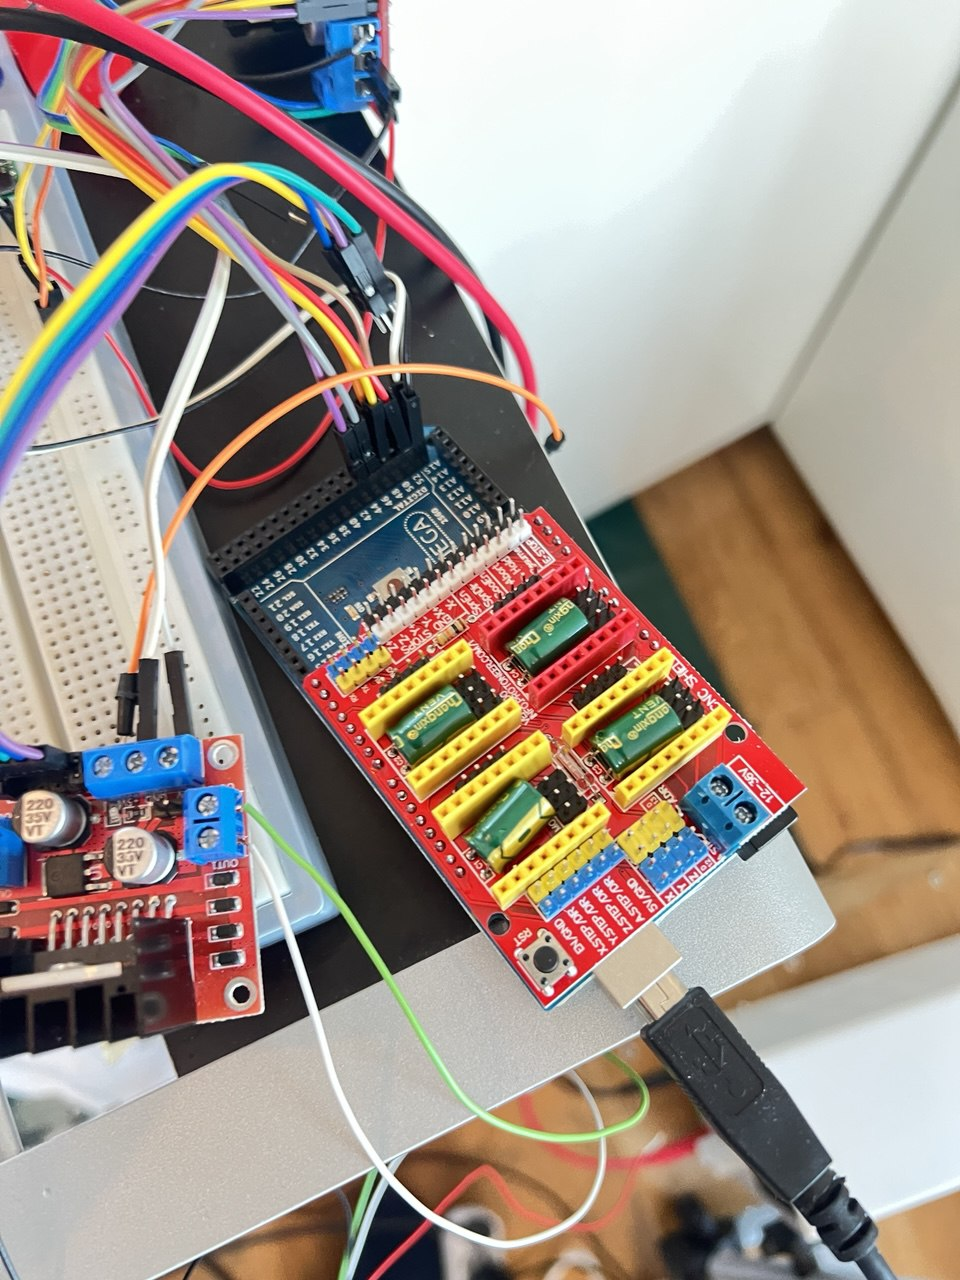
\includegraphics[width=.3\linewidth]{../photos/cnc_shield}
    \caption{CNC Shield}
    \label{fig:cnc_shield}
\end{figure}
\subsection{IR Distance Sensor}\label{subsec:ir-distance-sensor}
I use the GP2Y0E03\autocite{ir-sensor} infrared sensor, which, as the name suggests, uses Infrared red rays to measure the distance between the side of the table and the player.
This is done by emitting a short pulse with a photo diode and then measuring the time it took to reflect of the player and come back to the sensor, dividing the measured time by the speed of light and by two seconds, yields the distance.
The sensor outputs this distance either as a digital signal with the I2C protocol or as voltage difference, also called analog output.
As the digital output does not have a high resolution, the analog output is used, as it has a nearly 10x resolution.
But higher resolution does not automatically mean higher accuracy and that was also confirmed by the data I collected.
Luckily, the data seems to follow a binomial distribution, so by taking the average of $\approx100$ values, the program gets a good estimate of the actual value.
The integration of the measured data is relatively straight-forward, after moving to a specific position, the real distance is compared to the target distance and then the difference is corrected for.
This process is repeated roughly $5-10$ times, which often results in a back-and-forth motion, but the positions get more accurate with each iteration.

\subsection{Arduino code}\label{subsec:arduino-code}
Why do I use c++ for the code running on the arduino?
Usually I want to write all my code in rust, as it is a memory safe language and has a lot of other advantages, because it is quite new and has a lot of modern features.
One feature is the ease of importing other libraries, which in rust are called crates, which is not as easy in c++.
There is an arduino framework for rust, but I had problems with the serial connection, I couldn't get it to work reliably.
Therefore, I switched back to the default arduino framework, which is written in c++.
At first, I had a complex encoding scheme, which encoded all commands in different bytecodes.
However, then I realised that it was just simpler to send an integer for the position and, for example, a capital \("\)R\("\) for the reset command.
Implementing that in c++ for the arduino was quite easy, as the arduino framework has a lot of built-in functions for serial communication.